%!TEX program = xelatex
%!TEX root = ../all.tex

\chapter{Discriminative probabilistic classification}

\section*{Generalized linear models}

In the classification and regression settings considered so far, a recurring structural pattern has emerged. In particular, we have seen that posterior class distributions such as $p(C_k|\x)$ often take the form of a sigmoid (in the binary case) or a softmax (in the multiclass case), with arguments given by linear combinations of the input features. This observation is not accidental: it reflects a much more general modeling principle known as the framework of \alert{generalized linear models} (GLMs).

At a high level, GLMs provide a unifying language that connects linear predictors, probabilistic modeling, and nonlinear response functions. They explain why linear decision boundaries arise so naturally in a wide variety of learning problems, even when the predicted quantities themselves are probabilities or expectations rather than raw real-valued outputs.

\medskip
%\noindent\textbf{Definition of a GLM.}
A \alert{generalized linear model} is a function of the form
\begin{myequation}
h(\x)=f(\w^{T}\x+b)=f(\ow^{T}\ox),
\end{myequation}
where $\ox=(1,\x^{T})^{T}$ denotes the augmented feature vector, $\ow=(b,\w^{T})^{T}$ is the corresponding parameter vector, and $f$ is a generally nonlinear function known as the \emph{response function} or \emph{link function}. The role of $f$ is to map the linear predictor $\ow^{T}\ox$, which takes values in $\mathbb{R}$, to a range that is appropriate for the quantity being predicted (for example, $(0,1)$ for probabilities or $[0,\infty)$ for rates).

Despite the presence of a nonlinear response function, GLMs retain a crucial geometric property inherited from linear models. To see this, consider an iso-surface of the function $h(\x)$, defined by the condition
\begin{myequation}
h(\x)=c
\end{myequation}
for some constant $c$. By definition, this implies
\begin{myequation}
f(\ow^{T}\ox)=c.
\end{myequation}
Assuming that $f$ is invertible (as is the case for the standard GLM choices), we can apply $f^{-1}$ to both sides and obtain
\begin{myequation}
\ow^{T}\ox=f^{-1}(c)=c',
\end{myequation}
where $c'$ is another constant. This equation defines a hyperplane in the feature space. Therefore, \emph{all iso-surfaces of a GLM are hyperplanes}, and in particular all decision boundaries induced by thresholding a GLM are linear. This observation explains why many classifiers that appear nonlinear at the level of probabilities still yield linear decision boundaries in the input space.

\subsubsection*{Exponential families and GLMs}

The connection between GLMs and probability theory becomes precise once we consider conditional distributions belonging to the \alert{exponential family}. Suppose we wish to predict a random variable $t$ as a function of a set of explanatory variables $\x$. A prediction model for this task is a GLM if the following conditions hold.

First, the conditional distribution $p(t\mid\x)$ belongs to the exponential family. That is, it can be written in the form
\begin{myequation}
p(t|\x)=\frac{1}{s}\, g(\Vtheta(\x))\, f\!\left(\frac{t}{s}\right)
\exp\!\left(\frac{1}{s}\Vtheta(\x)^{T}\mathbf{u}(t)\right),
\end{myequation}
for suitable functions $g$, $f$, and $\mathbf{u}$, where $\Vtheta(\x)$ is the \alert{natural parameter} and $s$ is a scale parameter. This representation encompasses a wide range of commonly used distributions, including the normal, Bernoulli, categorical, Poisson, and exponential distributions.

Second, the goal of prediction is not necessarily to estimate $t$ directly, but rather to predict the conditional expectation of the \alert{sufficient statistics} $\mathbf{u}(t)$ given $\x$, namely $\mathbb{E}[\mathbf{u}(t)|\x]$.

Third, and most importantly for the GLM structure, the natural parameter $\Vtheta(\x)$ is assumed to depend linearly on the features:
\begin{myequation}
\Vtheta(\x)=\ow^{T}\ox.
\end{myequation}
Under these assumptions, the resulting predictor $h(\x)$ necessarily takes the form of a generalized linear model, with the response function determined by the choice of distribution in the exponential family.

\subsubsection*{GLM and normal distribution}

We begin with the simplest and most familiar case. Assume that $t\in\mathbb{R}$ and that the conditional distribution of $t$ given $\x$ is Gaussian:
\begin{myequation}
p(t|\x)=\frac{1}{\sqrt{2\pi}\sigma}
\exp\!\left(-\frac{(t-\mu(\x))^{2}}{2\sigma^{2}}\right),
\end{myequation}
with mean $\mu(\x)$ and constant variance $\sigma^{2}$. 

\medskip
In order to check that the Gaussian belongs to the exponential family, 
recall the exponential-family form introduced above:
\begin{myequation}
p(t|\x)=\frac{1}{s}\, g(\Vtheta(\x))\, f\!\left(\frac{t}{s}\right)\,
\exp\!\left(\frac{1}{s}\Vtheta(\x)^{T}\mathbf{u}(t)\right),
\end{myequation}

We need to rewrite its density so that the dependence on $t$ appears inside the exponential as a linear combination of fixed functions of $t$.

Starting from the Gaussian exponent, we have
\begin{myequation}
-\frac{(t-\mu(\x))^{2}}{2\sigma^{2}}
=-\frac{1}{2\sigma^{2}}\bigl(t^{2}-2t\mu(\x)+\mu(\x)^{2}\bigr)
=-\frac{t^{2}}{2\sigma^{2}}+\frac{\mu(\x)}{\sigma^{2}}\,t-\frac{\mu(\x)^{2}}{2\sigma^{2}}.
\end{myequation}
Substituting this back into the density yields
\begin{myequation}
p(t|\x)=\frac{1}{\sqrt{2\pi}\sigma}
\exp\!\left(-\frac{t^{2}}{2\sigma^{2}}\right)
\exp\!\left(\frac{\mu(\x)}{\sigma^{2}}\,t\right)
\exp\!\left(-\frac{\mu(\x)^{2}}{2\sigma^{2}}\right).
\end{myequation}

To match the general definition above, we can take (in this case $s=1$)
\begin{myequation}
\mathbf{u}(t)=
\begin{pmatrix}
t\\
t^{2}
\end{pmatrix},
\qquad
\Vtheta(\x)=
\begin{pmatrix}
\theta_{1}(\x)\\
\theta_{2}
\end{pmatrix}
=
\begin{pmatrix}
\mu(\x)/\sigma^{2}\\
-1/(2\sigma^{2})
\end{pmatrix}.
\end{myequation}
Then the exponent can be written compactly as
\begin{myequation}
\Vtheta(\x)^{T}\mathbf{u}(t)
=\theta_{1}(\x)\,t+\theta_{2}\,t^{2}
=\frac{\mu(\x)}{\sigma^{2}}\,t-\frac{1}{2\sigma^{2}}\,t^{2},
\end{myequation}
which reproduces exactly the two $t$-dependent exponential factors above. The remaining terms can be identified as
\begin{myequation}
f(t)=\frac{1}{\sqrt{2\pi}\sigma}\exp\!\left(-\frac{t^{2}}{2\sigma^{2}}\right),
\qquad
g(\Vtheta(\x))=\exp\!\left(-\frac{\mu(\x)^{2}}{2\sigma^{2}}\right),
\qquad s=1,
\end{myequation}
so that indeed
\begin{myequation}
p(t|\x)=g(\Vtheta(\x))\, f(t)\, \exp\!\bigl(\Vtheta(\x)^{T}\mathbf{u}(t)\bigr).
\end{myequation}
This explicit identification shows in detail why the Gaussian density can be written in exponential-family form.

\medskip

In this representation the sufficient statistic is the vector $\mathbf{u}(t)=(t,t^{2})^{T}$. In the GLM construction discussed earlier, the quantity we ultimately wish to predict is the conditional mean $\mathbb{E}[t\mid\x]=\mu(\x)$, which is tied specifically to the first component $\theta_{1}(\x)$. This is why, in the subsequent derivation, it is common to emphasize the relationship between $\theta_{1}(\x)$ and $\mu(\x)$, while $\theta_{2}$ remains constant because the variance $\sigma^{2}$ is assumed fixed.




If our goal is to predict the conditional expectation
\begin{myequation}
\mathbb{E}[t|\x]=\mu(\x),
\end{myequation}
we identify $h(\x)=\mu(\x)$. Since $\mu(\x)=\sigma^{2}\theta_{1}(\x)$, we obtain
\begin{myequation}
h(\x)=\sigma^{2}\theta_{1}(\x).
\end{myequation}
Finally, assuming that $\theta_{1}(\x)$ is a linear function of the features, $\theta_{1}(\x)=\ow^{T}\ox$, we arrive at
\begin{myequation}
h(\x)=\sigma^{2}\ow^{T}\ox,
\end{myequation}
which is simply linear regression. Thus, ordinary least-squares regression appears as a special case of the GLM framework associated with the normal distribution and the identity link function.

\subsubsection*{GLM and Bernoulli distribution}

We now turn to the case of \emph{binary outcomes}, which plays a central role in classification problems and provides a particularly clear illustration of the generalized linear model framework. In this setting, the target variable can take only two values, and the goal of learning is to estimate the probability that an observation belongs to one of the two possible classes.

\medskip
Assume that $t\in\{0,1\}$ and that the conditional distribution of $t$ given the input features $\x$ is Bernoulli:
\begin{myequation}
p(t|\x)=\pi(\x)^{t}(1-\pi(\x))^{1-t},
\end{myequation}
where $\pi(\x)=p(t=1\mid\x)$ denotes the probability of the positive class. This compact expression encodes both possible outcomes: when $t=1$, the likelihood reduces to $\pi(\x)$; when $t=0$, it reduces to $1-\pi(\x)$. As in the Gaussian case, the Bernoulli distribution belongs to the exponential family, which makes it amenable to a systematic GLM treatment.

To make this explicit, recall that exponential-family distributions are characterized by a natural parameter and a sufficient statistic. For the Bernoulli distribution, the sufficient statistic is simply
\begin{myequation}
\mathbf{u}(t)=t,
\end{myequation}
reflecting the fact that all information about the outcome is contained in whether the event occurred or not. The corresponding natural parameter is given by
\begin{myequation}
\theta(\x)=\log\frac{\pi(\x)}{1-\pi(\x)},
\end{myequation}
which is known as the \alert{log-odds} or \alert{logit}. This quantity measures, on a logarithmic scale, how much more likely the positive outcome $t=1$ is compared to the negative outcome $t=0$. Unlike $\pi(\x)$, which is constrained to lie in the interval $(0,1)$, the log-odds $\theta(\x)$ can take any real value, making it a natural candidate for a linear predictor.

\medskip
%\noindent\textbf{Prediction and the response function.}
In the GLM framework, the quantity we aim to predict is typically the conditional expectation of the sufficient statistic. In the Bernoulli case this expectation is
\begin{myequation}
\mathbb{E}[t\mid\x]=\pi(\x),
\end{myequation}
which coincides with the probability of the positive class. The relationship between this expectation and the natural parameter $\theta(\x)$ is obtained by inverting the log-odds transformation. Solving
\begin{myequation}
\theta(\x)=\log\frac{\pi(\x)}{1-\pi(\x)}
\end{myequation}
for $\pi(\x)$ yields
\begin{myequation}
h(\x)=\pi(\x)=\frac{1}{1+e^{-\theta(\x)}},
\end{myequation}
which is the \alert{logistic} or \alert{sigmoid} function. This function maps any real-valued input to the interval $(0,1)$, ensuring that the model outputs are valid probabilities. Its smooth, S-shaped form reflects a gradual transition between the two classes as the underlying score $\theta(\x)$ changes sign.

\medskip
%\noindent\textbf{Logistic regression as a GLM.}
To complete the construction of the model, we now impose the defining assumption of generalized linear models: the natural parameter is a linear function of the features. Specifically, we assume
\begin{myequation}
\theta(\x)=\ow^{T}\ox,
\end{myequation}
where $\ox$ is the augmented feature vector and $\ow$ is the parameter vector. Substituting this expression into the response function yields
\begin{myequation}
h(\x)=\frac{1}{1+e^{-\ow^{T}\ox}},
\end{myequation}
which is precisely the functional form of \alert{logistic regression}.

This derivation highlights an important conceptual point. Logistic regression does not arise as an arbitrary choice of a sigmoid applied to a linear score. Rather, it is the natural consequence of combining three ingredients: a Bernoulli model for the target variable, the exponential-family representation of that model, and the GLM assumption that the natural parameter depends linearly on the input features. From this perspective, logistic regression inherits both a clear probabilistic interpretation and the geometric simplicity of linear decision boundaries, making it a cornerstone method for binary classification.


\subsubsection*{GLM and categorical distribution}

The Bernoulli case discussed previously extends in a natural and conceptually straightforward way to situations in which the target variable can take more than two discrete values. This setting arises whenever we are faced with a multiclass classification problem, where each observation must be assigned to one among $K>2$ possible classes.

\medskip
%\noindent\textbf{Categorical outcomes and one-hot encoding.}
Assume that the target variable $t$ takes values in the finite set $\{1,\ldots,K\}$. A convenient representation of such a variable is given by the so-called \emph{one-hot} (or 1-of-$K$) encoding: for each realization $t$, we define a vector $(t_1,\ldots,t_K)$ such that
\begin{myequation}
t_i =
\begin{cases}
1 & \text{if } t=i,\\
0 & \text{otherwise}.
\end{cases}
\end{myequation}
Under this representation, the conditional distribution of $t$ given $\x$ can be written as
\begin{myequation}
p(t|\x)=\prod_{i=1}^{K}\pi_{i}(\x)^{t_i},
\end{myequation}
where $\pi_i(\x)=p(t=i\mid\x)$ denotes the posterior probability of class $i$. This is the \alert{categorical distribution}, which generalizes the Bernoulli distribution to the case of multiple mutually exclusive outcomes. The parameters $\pi_1(\x),\ldots,\pi_K(\x)$ satisfy the normalization constraint
\begin{myequation}
\sum_{i=1}^{K}\pi_i(\x)=1,
\end{myequation}
reflecting the fact that exactly one class must occur.

\medskip
%\noindent\textbf{Exponential-family form and natural parameters.}
The categorical distribution belongs to the exponential family, and this fact allows it to be embedded naturally into the GLM framework. In particular, its natural parameter vector can be written as
\begin{myequation}
\Vtheta(\x)=(\theta_1(\x),\ldots,\theta_K(\x))^{T},
\end{myequation}
with components defined by
\begin{myequation}
\theta_{i}(\x)=\log\frac{\pi_i(\x)}{\pi_K(\x)}
=\log\frac{\pi_i(\x)}{1-\sum_{j=1}^{K-1}\pi_j(\x)}.
\end{myequation}
This parameterization deserves some interpretation. Rather than working directly with the probabilities $\pi_i(\x)$, which are constrained to be nonnegative and to sum to one, we work with unconstrained real-valued quantities $\theta_i(\x)$. Each $\theta_i(\x)$ represents the \emph{log-odds} of class $i$ relative to a reference class, here chosen to be class $K$. The choice of a reference class is arbitrary and does not affect the final model, but it removes redundancy and ensures identifiability of the parameters.

The sufficient statistic associated with this exponential-family representation is simply
\begin{myequation}
\mathbf{u}(t)=(t_1,\ldots,t_K)^T,
\end{myequation}
which mirrors the one-hot encoding of the class label.

\medskip
%\noindent\textbf{From natural parameters to predicted probabilities.}
As in the Bernoulli case, the quantity of interest for prediction is the conditional expectation of the sufficient statistics. Since $\mathbb{E}[t_i\mid\x]=p(t=i\mid\x)=\pi_i(\x)$, the GLM predictor for class $i$ is
\begin{myalign}
h_i(\x)=\pi_i(\x).
\end{myalign}
Using the definition of the natural parameters, we can express these probabilities in terms of $\theta_i(\x)$. From
\begin{myequation}
\theta_i(\x)=\log\frac{\pi_i(\x)}{\pi_K(\x)},
\end{myequation}
we obtain
\begin{myequation}
\pi_i(\x)=\pi_K(\x)e^{\theta_i(\x)}.
\end{myequation}
To determine $\pi_K(\x)$, we impose the normalization condition $\sum_{i=1}^{K}\pi_i(\x)=1$, which yields
\begin{myequation}
\pi_K(\x)\sum_{i=1}^{K}e^{\theta_i(\x)}=1.
\end{myequation}
Solving for $\pi_K(\x)$ and substituting back gives the familiar expressions
\begin{myequation}
\pi_{K}(\x)=\frac{1}{\sum_{i=1}^{K}e^{\theta_{i}(\x)}},
\qquad
\pi_{i}(\x)=\frac{e^{\theta_{i}(\x)}}{\sum_{j=1}^{K}e^{\theta_{j}(\x)}}.
\end{myequation}
These equations show how a set of unconstrained real-valued scores $\theta_i(\x)$ is transformed into a valid probability distribution over classes.

\medskip
%\noindent\textbf{Softmax regression as a GLM.}
To complete the GLM construction, we assume that each natural parameter is a linear function of the features,
\begin{myequation}
\theta_i(\x)=\ow_i^{T}\ox,
\end{myequation}
where $\ox$ denotes the augmented feature vector and $\ow_i$ is the parameter vector associated with class $i$. Substituting this assumption into the expressions above yields
\begin{myalign}
h_i(\x)&=\frac{e^{\ow_{i}^{T}\ox}}{\sum_{j=1}^{K}e^{\ow_{j}^{T}\ox}},
\qquad i=1,\ldots,K-1,\\
h_K(\x)&=\frac{1}{\sum_{j=1}^{K}e^{\ow_{j}^{T}\ox}}.
\end{myalign}
This model is known as \alert{softmax regression}. It is the direct multiclass generalization of logistic regression and arises naturally as the generalized linear model associated with categorical outcomes.

\medskip
From a geometric perspective, each linear score $\ow_i^{T}\ox$ defines a hyperplane in feature space, and classification is based on comparing these scores across classes. From a probabilistic perspective, the softmax function ensures that the outputs form a coherent probability distribution. The GLM derivation thus clarifies that softmax classifiers are not ad hoc constructions, but rather the principled result of combining linear predictors with the exponential-family model for categorical data.


\subsubsection*{GLM and additional regressions}

The framework of generalized linear models (GLMs) extends well beyond the most familiar cases of linear regression and logistic classification. Its real strength lies in the possibility of modeling a wide variety of response variables simply by selecting an appropriate member of the exponential family and linking its natural parameter to a linear predictor. In this way, GLMs offer a principled and flexible approach to regression problems involving non-Gaussian data, such as counts, waiting times, or other constrained responses.

\paragraph*{Poisson distribution.}
We begin by considering the case in which the target variable $t \in \{0,1,\ldots\}$ takes nonnegative integer values, as is typical in count data (for instance, the number of events occurring in a fixed time interval). A natural probabilistic model for such data is the Poisson distribution, whose conditional density is given by
\begin{myequation}
p(t|\x) = \frac{\lambda(\x)^t}{t!} e^{-\lambda(\x)},
\end{myequation}
where $\lambda(\x) > 0$ denotes the rate parameter and may depend on the input $\x$.

Written in exponential-family form, the Poisson distribution has natural parameter
\begin{myequation}
\theta(\x) = \log \lambda(\x),
\end{myequation}
and sufficient statistic $\mathbf{u}(t) = t$. This representation makes explicit the logarithmic link between the mean parameter $\lambda(\x)$ and the natural parameter $\theta(\x)$. One immediate consequence of this formulation is that the conditional expectation of the response is
\begin{myequation}
\mathbb{E}[t|\x] = \lambda(\x),
\end{myequation}
which coincides with the rate parameter itself. Therefore, if the goal of prediction is to estimate the conditional mean, the corresponding response function takes the form
\begin{myequation}
h(\x) = \lambda(\x) = e^{\theta(\x)}.
\end{myequation}
This exponential relationship is not arbitrary: it arises directly from the structure of the exponential family and ensures that the predicted mean remains strictly positive, as required for count data.

By assuming a linear model for the natural parameter,
\begin{myequation}
\theta(\x) = \ow^{T} \ox,
\end{myequation}
we obtain the standard Poisson regression model,
\begin{myequation}
h(\x) = e^{\ow^{T} \ox}.
\end{myequation}
In this setting, the exponential function acts as the canonical link, transforming the linear predictor into a valid mean parameter. Poisson regression thus provides a clear example of how GLMs combine linear structure with nonlinear response functions in a principled way.

\paragraph*{Exponential distribution.}
As a second example, consider the case in which the target variable $t \in [0,\infty)$ is a nonnegative real-valued quantity. This situation commonly arises when modeling waiting times or durations between events. A simple and widely used model for such data is the exponential distribution, whose conditional density is
\begin{myequation}
p(t|\x) = \lambda(\x) e^{-\lambda(\x) t},
\end{myequation}
with rate parameter $\lambda(\x) > 0$.

In exponential-family form, the natural parameter is
\begin{myequation}
\theta(\x) = -\lambda(\x),
\end{myequation}
and the sufficient statistic is again $\mathbf{u}(t) = t$. Unlike the Poisson case, the natural parameter here is negative, reflecting the fact that the exponential distribution decays with increasing $t$. The conditional expectation of the response is
\begin{myequation}
\mathbb{E}[t|\x] = \frac{1}{\lambda(\x)} = -\frac{1}{\theta(\x)}.
\end{myequation}
If we once more adopt the perspective that prediction should target the conditional mean, the resulting response function is
\begin{myequation}
h(\x) = -\frac{1}{\theta(\x)}.
\end{myequation}
This inverse relationship between the mean and the natural parameter highlights a different type of nonlinearity compared to the Poisson case, but it is equally dictated by the probabilistic structure of the model.

Assuming a linear dependence of the natural parameter on the input,
\begin{myequation}
\theta(\x) = \ow^{T} \ox,
\end{myequation}
we arrive at exponential regression,
\begin{myequation}
h(\x) = -\frac{1}{\ow^{T} \ox}.
\end{myequation}
Here, the linear predictor must be constrained so that $\ow^{T} \ox < 0$, ensuring a positive rate parameter and a well-defined mean. This example further illustrates how GLMs naturally encode domain constraints through the choice of link function.

\medskip
In conclusion, generalized linear models provide a coherent and unifying framework in which many classical regression and classification techniques emerge as special cases. By coupling linear predictors with response functions derived systematically from exponential-family distributions, GLMs reconcile probabilistic modeling with geometric simplicity. This perspective clarifies why linear decision boundaries and linear predictors appear so ubiquitously in learning problems, even when the observed data exhibit highly non-Gaussian behavior.



%
%%%%%%%%%%%Logistic regression
%
\section*{Discriminative approach}

Within the discriminative approach, the focus is placed directly on modeling the posterior class probabilities $ p(C_k|\x) $, rather than on the joint distribution of inputs and labels. In other words, instead of asking how the data are generated within each class, we are primarily interested in how the class labels depend on the observed input $\x$. A common and effective assumption is that these posterior probabilities can be expressed within the framework of generalized linear models (GLMs), whose parameters are then estimated from data, typically through maximum likelihood methods.

This perspective leads to a conceptual shift with respect to the generative approach. Since the conditional distribution $p(\x|C_k)$ is not modeled, the discriminative strategy inevitably provides less information about the data-generating process as a whole. For instance, it does not allow the generation of new synthetic samples conditioned on a class label. However, this loss of information is often compensated by a substantial simplification of the model: fewer parameters are involved, and fewer assumptions about the structure of the data are required. As a result, discriminative models are often easier to train and, crucially, can yield superior predictive performance when the assumptions underlying generative models—such as Gaussian class-conditional densities—are violated or poorly matched to the true data distribution.

\subsection*{Logistic regression}

A paradigmatic example of the discriminative approach is \alert{logistic regression}. This model arises naturally as a GLM under the assumption that the target variable $t$, encoding class membership, follows a Bernoulli distribution. In the binary classification setting, where $C_1$ denotes the positive class, this assumption leads to the posterior probability
\begin{myequation}
p(C_{1}|\x) = \sigma(\ow^{T}\ox) = \frac{1}{1 + e^{-\ow^{T}\ox}},
\end{myequation}
where $\sigma(\cdot)$ is the logistic sigmoid function. As usual, the vector $\ox$ may include a constant component to account for the bias term, and more generally it may consist of nonlinear basis functions of the original input variables.

The use of the sigmoid function is not arbitrary: it is the canonical response function associated with the Bernoulli distribution in the GLM framework. It maps the linear predictor $\ow^{T}\ox$, which can take any real value, into the interval $(0,1)$, ensuring that the output can be consistently interpreted as a probability. In this sense, logistic regression for classification plays a role analogous to that of linear regression for real-valued targets, differing only in the assumed distribution of the response variable and the corresponding link function.

\subsubsection*{Degrees of freedom}

An important practical distinction between discriminative and generative approaches concerns the number of parameters that must be estimated from the data. In logistic regression, the model requires the estimation of $d+1$ coefficients: the bias term $b$ and the weights $w_1, \ldots, w_d$ associated with the $d$-dimensional input.

By contrast, a generative approach based on Gaussian class-conditional densities typically involves a significantly larger number of parameters. For a binary classification problem, two mean vectors $\Vmu_1$ and $\Vmu_2$ must be estimated, contributing a total of $2d$ parameters. In addition, each covariance matrix introduces
\begin{myequation}
\sum_{i=1}^{d} i = \frac{d(d+1)}{2}
\end{myequation}
independent coefficients, reflecting the symmetry of the covariance matrix. Finally, one must estimate the prior class probability $p(C_1)$.

Altogether, this results in $d(d+1) + 2d + 1 = d(d+3) + 1$ parameters when distinct covariance matrices are assumed for each class. Even under the simplifying assumption of a shared covariance matrix, the total number of parameters remains $d(d+1)/2 + 2d + 1 = d(d+5)/2 + 1$, which can be substantially larger than the number required by logistic regression. This difference highlights why discriminative models are often preferable in high-dimensional settings or when training data are limited.

\subsubsection*{Maximum likelihood estimation}

To estimate the parameters of logistic regression, we adopt a maximum likelihood perspective. As stated above, we assume that the target associated with each training example follows a Bernoulli distribution conditioned on the input and the model parameters. Formally, for each training pair $(\x_i, t_i)$, we write
\begin{myequation}
p(t_i|\x_i; \w) = p_i^{t_i}(1 - p_i)^{1 - t_i},
\end{myequation}
where
\begin{myequation}
p_i = p(C_1|\x_i) = \sigma(a_i), \qquad a_i = \ow^{T}\ox_i.
\end{myequation}

Assuming independence across training samples, the likelihood of the entire set of targets $\t$ given the inputs $\X$ is
\begin{myequation}
p(\t|\X; \ow) = L(\ow|\X, \t) = \prod_{i=1}^{n} p_i^{t_i}(1 - p_i)^{1 - t_i}.
\end{myequation}
Taking the logarithm, which simplifies both analysis and computation, yields the log-likelihood
\begin{myequation}
l(\ow|\X, \t) = \log L(\ow|\X, \t) = \sum_{i=1}^{n} \left( t_i \log p_i + (1 - t_i) \log (1 - p_i) \right).
\end{myequation}

To maximize this objective function, we compute its gradient with respect to the model parameters. Applying the chain rule, we obtain
\begin{myalign}
\frac{\partial l}{\partial w_j}
&= \sum_{i=1}^{n}
\frac{\partial \log p(\ow|\x_i, t_i)}{\partial p_i}
\frac{\partial p_i}{\partial a_i}
\frac{\partial a_i}{\partial w_j}.
\end{myalign}
Each term in this expression can be computed explicitly. In particular,
\begin{myalign}
\frac{\partial \log p(\ow|\x_i, t_i)}{\partial p_i}
&= \frac{t_i}{p_i} - \frac{1 - t_i}{1 - p_i}
= \frac{t_i - p_i}{p_i(1 - p_i)}, \\
\frac{\partial p_i}{\partial a_i}
&= \frac{\partial \sigma(a_i)}{\partial a_i}
= \sigma(a_i)(1 - \sigma(a_i))
= p_i(1 - p_i), \\
\frac{\partial a_i}{\partial w_j}
&= x_{ij}.
\end{myalign}
Combining these terms leads to a substantial simplification, since the factors $p_i(1 - p_i)$ cancel out. As a result, we find
\begin{myalign}
\frac{\partial}{\partial w_j} l(\ow|\X, \t)
&= \sum_{i=1}^{n} (t_i - p_i) x_{ij}
= \sum_{i=1}^{n} \bigl(t_i - \sigma(\ow^{T}\ox_i)\bigr) x_{ij}.
\end{myalign}
A similar argument applies to the derivative with respect to the bias term $b$, noting that $\partial a_i / \partial b = 1$, which gives
\begin{myalign}
\frac{\partial}{\partial b} l(\ow|\X, \t)
&= \sum_{i=1}^{n} (t_i - \sigma(\ow^{T}\ox_i)).
\end{myalign}

In compact vector notation, the gradient of the log-likelihood can be written as
\begin{myalign}
\nabla_{\ow} l(\ow|\X, \t)
&= \sum_{i=1}^{n} (t_i - \sigma(\ow^{T}\ox_i)) \ox_i.
\end{myalign}
This expression admits a clear interpretation: each training example contributes an update proportional to the difference between the observed label and the predicted probability, weighted by the input vector.

To maximize the likelihood, one can apply a gradient ascent algorithm. Starting from an initial guess $\ow^{(0)}$, the parameters are iteratively updated according to
\begin{myalign}
\ow^{(j+1)}
&= \ow^{(j)} + \alpha \nabla_{\ow} l(\ow|\X, \t)\big|_{\ow^{(j)}} \\
&= \ow^{(j)} + \alpha \sum_{i=1}^{n} \bigl(t_i - \sigma((\ow^{(j)})^{T}\ox_i)\bigr) \ox_i \\
&= \ow^{(j)} + \alpha \sum_{i=1}^{n} \bigl(t_i - h^{(j)}(\x_i)\bigr) \ox_i,
\end{myalign}
where $\alpha > 0$ denotes the learning rate.

As an alternative to updating all components of $\ow$ simultaneously, one may consider updating a single coefficient at a time. In this coordinate-wise scheme, the update rule for the $k$-th component becomes
\begin{align*}
w_k^{(j+1)}
&= w_k^{(j)} + \alpha \frac{\partial l(\w|\X, \t)}{\partial w_k}\big|_{\w^{(j)}} \\
&= w_k^{(j)} + \alpha \sum_{i=1}^{n} \bigl(t_i - \sigma((\w^{(j)})^{T}\overline{\x}_i)\bigr) x_{ik} \\
&= w_k^{(j)} + \alpha \sum_{i=1}^{n} \bigl(t_i - y(\x_i)\bigr) x_{ik}.
\end{align*}
Both strategies exploit the same underlying gradient structure and illustrate how logistic regression combines probabilistic modeling with efficient optimization procedures.

\medskip
\subsubsection*{Regularization effects}

In practical applications, logistic regression models are often augmented with a regularization term. As usual, the most common choice is $\ell_2$ (ridge) regularization, which adds a quadratic penalty to the negative log-likelihood. In this case, instead of maximizing the log-likelihood $l(\ow|\X, \t)$, one maximizes the regularized objective
\begin{myequation}
l_{\text{reg}}(\ow|\X, \t)
= l(\ow|\X, \t) - \frac{\lambda}{2} \|\ow\|^2,
\end{myequation}
where $\lambda > 0$ is a regularization parameter controlling the strength of the penalty. This formulation, we already observed,  admits a clear Bayesian interpretation: it corresponds to assuming a zero-mean isotropic Gaussian prior over the parameters $\ow$, with variance inversely proportional to $\lambda$.

From the standpoint of learning, regularization directly modifies the gradient of the objective function. For $\ell_2$ regularization, the gradient of the regularized log-likelihood becomes
\begin{myequation}
\nabla_{\ow} l_{\text{reg}}(\ow|\X, \t)
= \sum_{i=1}^{n} (t_i - \sigma(\ow^{T}\ox_i)) \ox_i - \lambda \ow.
\end{myequation}
Compared to the unregularized case, an additional term proportional to $-\ow$ appears, which continuously pulls the parameters toward the origin during gradient ascent. The corresponding update rule thus takes the form
\begin{myequation}
\ow^{(j+1)}
= \ow^{(j)} + \alpha \left[ \sum_{i=1}^{n} (t_i - \sigma((\ow^{(j)})^{T}\ox_i)) \ox_i - \lambda \ow^{(j)} \right].
\end{myequation}
This update can be interpreted as a combination of a data-driven correction, derived from the prediction errors, and a shrinkage term that counteracts weight growth.

An alternative and widely used form of regularization is $\ell_1$ regularization, which penalizes the sum of the absolute values of the parameters. While the corresponding objective function is no longer differentiable everywhere, its effect on the model is qualitatively different: it promotes sparsity in the solution, driving many components of $\ow$ exactly to zero. As a consequence, $\ell_1$-regularized logistic regression can be interpreted as performing implicit feature selection, which is particularly advantageous when only a small subset of input variables is truly informative.


\subsection*{Second order methods for likelihood maximization}

We now turn to second-order optimization methods and show how the Newton--Raphson method can be applied to logistic regression. This development leads naturally to a well-known algorithm in statistical learning, the \alert{Iteratively Reweighted Least Squares} (IRLS) method. Compared to first-order approaches such as gradient ascent, Newton--Raphson exploits curvature information of the objective function and often converges in significantly fewer iterations.

To introduce the method, consider first the scalar case. Given a function $ f : \mathbb{R} \to \mathbb{R} $, the Newton--Raphson algorithm aims at finding a value $ z \in \mathbb{R} $ such that $ f(z) = 0 $. Starting from an initial guess $ z_0 $, the algorithm generates a sequence of iterates according to
\begin{myequation}
z_{j+1} = z_j - \frac{f(z_j)}{f'(z_j)}.
\end{myequation}
At each iteration, the function $ f $ is locally approximated by its first-order Taylor expansion, that is, by the line tangent to the graph of $ f $ at the point $ (z_j, f(z_j)) $. The next iterate $ z_{j+1} $ is then defined as the point where this tangent line intersects the horizontal axis. This geometric interpretation explains both the efficiency of the method near a solution and its potential sensitivity to the choice of the initial point.

\begin{center}

\includegraphics[width=0.7\textwidth]{newton.pdf}
\end{center}

The Newton--Raphson method can also be used to find maxima or minima of a function. In this case, one applies the algorithm to the derivative $ f'(z) $, so that stationary points are found by solving $ f'(z) = 0 $. The resulting update rule takes the form
\begin{myequation}
z_{j+1} = z_j - \frac{f'(z_j)}{f''(z_j)},
\end{myequation}
where the second derivative $ f''(z_j) $ encodes local curvature information. When $ f $ is twice differentiable and locally well approximated by a quadratic function, this update can lead to very rapid convergence.

To apply Newton--Raphson to logistic regression, we must extend these ideas to the multivariate case, since the optimization problem involves the vector of parameters $ \w $. In this setting, the first derivative is replaced by the gradient $ \nabla_{\w} $, while the second derivative generalizes to the \alert{Hessian matrix} $ \H $, whose entries are defined as
\begin{myequation}
\H_{ij}(f) = \frac{\partial^2 f}{\partial w_i \partial w_j}.
\end{myequation}
The Newton--Raphson update rule for maximizing a function $ f(\w) $ then becomes
\begin{myequation}
\ow^{(j+1)} = \ow^{(j)} - \left( \H(f)\big|_{\ow^{(j)}} \right)^{-1} \nabla_{\ow} f \big|_{\ow^{(j)}}.
\end{myequation}
This expression highlights the key difference with respect to gradient-based methods: the update direction is scaled by the inverse Hessian, effectively rescaling the gradient according to the local curvature of the objective function.

Before specializing to logistic regression, it is instructive to recall how Newton--Raphson behaves in the simpler case of linear regression. Here, the error function to be minimized is the squared error
\begin{myequation}
E(\ow) = \frac{1}{2} \sum_{i=1}^{n} \bigl( h(\x_i) - t_i \bigr)^2
= \frac{1}{2} \sum_{i=1}^{n} (\ow^{T}\ox_i - t_i)^2.
\end{myequation}
The gradient and Hessian of this error function are given by
\begin{myalign}
\nabla_{\ow} E
&= \sum_{i=1}^{n} (h(\x_i) - t_i)\ox_i
= \oX^{T}\oX\ow - \oX^{T}\t, \\
\H(E)
&= \nabla_{\ow}\nabla_{\ow} E
= \sum_{i=1}^{n} \ox_i \ox_i^{T}
= \oX^{T}\oX.
\end{myalign}
Substituting these expressions into the Newton--Raphson update yields
\begin{myalign}
\ow^{(j+1)}
&= \ow^{(j)} - (\oX^{T}\oX)^{-1}(\oX^{T}\oX\ow^{(j)} - \oX^{T}\t)
= (\oX^{T}\oX)^{-1}\oX^{T}\t.
\end{myalign}
Remarkably, the dependence on $ \ow^{(j)} $ disappears, and the algorithm converges in a single iteration to the well-known closed-form solution of linear regression. This behavior reflects the fact that the squared error is a quadratic function of $ \ow $, for which Newton--Raphson is exact.

The situation is more interesting in logistic regression, where the objective function is no longer quadratic. In this case, we minimize the \alert{cross-entropy} loss
\begin{myalign}
E(\ow)
&= -l(\ow \mid \X, \t)
= -\sum_{i=1}^{n} \left( t_i \log h(\x_i) + (1 - t_i)\log(1 - h(\x_i)) \right),
\end{myalign}
with $ h(\x_i) = \sigma(\ow^{T}\ox_i) $. The gradient of this loss function can be written as
\begin{myalign}
\nabla_{\ow} E
&= -\nabla_{\ow} l(\ow \mid \X, \t)
= \sum_{i=1}^{n} (h(\x_i) - t_i)\ox_i
= \oX^{T}(\y - \t),
\end{myalign}
where $ \y $ denotes the vector of predictions $ y_i = \sigma(\ow^{T}\ox_i) $. The Hessian matrix takes the form
\begin{myalign}
\H(E)
&= \sum_{i=1}^{n} y_i(1 - y_i)\ox_i \ox_i^{T}
= \oX^{T}\Y\oX,
\end{myalign}
where $ \Y $ is an $ n \times n $ diagonal matrix with entries
\begin{myequation}
Y_{ii} = y_i(1 - y_i).
\end{myequation}
The diagonal structure of $ \Y $ reflects the fact that each data point contributes independently to the curvature of the loss function, with a weight determined by the local slope of the sigmoid.

The Newton--Raphson update for logistic regression therefore becomes
\begin{myalign}
\ow^{(j+1)}
&= \ow^{(j)} - (\oX^{T}\Y^{(j)}\oX)^{-1}\oX^{T}(\y^{(j)} - \t),
\end{myalign}
where both $ \y^{(j)} $ and $ \Y^{(j)} $ depend on the current estimate $ \ow^{(j)} $. By adding and subtracting a suitable term, this update can be rewritten in a more revealing form:
\begin{myalign}
\ow^{(j+1)}
&= (\oX^{T}\Y^{(j)}\oX)^{-1}\oX^{T}\Y^{(j)}
\left( \oX\ow^{(j)} - {\Y^{(j)}}^{-1}(\y^{(j)} - \t) \right) \\
&= (\oX^{T}\Y^{(j)}\oX)^{-1}\oX^{T}\Y^{(j)} \z^{(j)},
\end{myalign}
where the vector
\begin{myequation}
\z^{(j)} = \oX\ow^{(j)} - {\Y^{(j)}}^{-1}(\y^{(j)} - \t)
\end{myequation}
is often referred to as the \emph{adjusted response}. It depends explicitly on the current parameter estimate and can be interpreted as a local linearization of the nonlinear classification problem.

At this point, the connection with weighted least squares becomes apparent. Consider the \alert{weighted least squares} cost function
\begin{myequation}
\sum_{i=1}^{n} \psi_i \bigl( \tilde h(\x_i) - \tilde t_i \bigr)^2
= \sum_{i=1}^{n} \psi_i (\tilde\ow^{T}\ox_i - \tilde t_i)^2,
\end{myequation}
where $ \psi_1, \ldots, \psi_n $ are nonnegative weights associated with the data points. Ordinary least squares is recovered as the special case $ \psi_i = 1 $ for all $ i $. It can be shown that the minimizer of this weighted problem admits the closed-form solution
\begin{myequation}
\tilde\w^{*} = (\oX^{T}\VPsi\oX)^{-1}\oX^{T}\VPsi \tilde\t,
\end{myequation}
where $ \VPsi $ is a diagonal matrix with entries $ \VPsi_{ii} = \psi_i $.

Comparing this expression with the Newton--Raphson update derived above, we see that each iteration of logistic regression optimization can be interpreted as solving a weighted least squares problem with
\begin{myequation}
\VPsi = \Y^{(j)}, \qquad \tilde\t = \z^{(j)}.
\end{myequation}
This observation provides the rationale for the name \alert{Iteratively Reweighted Least Squares}: at each iteration, the algorithm constructs a new weighted least squares problem, solves it in closed form, updates the parameter vector $ \ow^{(j+1)} $, and then recomputes the weights $ \VPsi = \Y^{(j+1)} $ and the adjusted targets $ \tilde\t = \z^{(j+1)} $.

In summary, the Newton--Raphson method applied to logistic regression leads to an elegant and powerful optimization procedure. By repeatedly approximating the nonlinear cross-entropy loss with a locally quadratic, weighted least squares problem, IRLS combines the fast convergence of second-order methods with the analytical simplicity of linear regression.

\subsubsection*{Logistic regression and GDA}

It is instructive to conclude the discussion on discriminative and generative classifiers by clarifying the precise relationship between logistic regression and Gaussian Discriminant Analysis (GDA). Although these two approaches are often presented as conceptually distinct, they are in fact closely connected, and understanding this connection helps to clarify both their strengths and their limitations.

Let us begin from the generative perspective. Suppose that the class-conditional densities $ p(\x \mid C_1) $ and $ p(\x \mid C_2) $ are modeled as multivariate normal distributions with means $ \Vmu_1 $ and $ \Vmu_2 $, respectively, and with a common covariance matrix $ \VSigma $. Under this assumption, Bayes’ rule can be applied to compute the posterior probability $ p(C_1 \mid \x) $. A direct calculation shows that the logarithm of the posterior odds ratio,
\begin{myequation}
\log \frac{p(C_1 \mid \x)}{p(C_2 \mid \x)},
\end{myequation}
is an affine (that is, linear plus constant) function of $ \x $. As a consequence, the posterior probability itself takes the logistic form
\begin{myequation}
p(C_1 \mid \x) = \sigma(\ow^{T}\ox),
\end{myequation}
for a suitable choice of the parameter vector $ \ow $, which depends on $ \Vmu_1 $, $ \Vmu_2 $, $ \VSigma $, and the class priors. This result shows that, under the Gaussian assumption with shared covariance, GDA induces exactly the same functional form for the posterior as logistic regression. In this sense, logistic regression can be seen as the discriminative counterpart of this particular generative model.

The converse implication, however, does not hold in general. Starting from a logistic posterior $ p(C_1 \mid \x) = \sigma(\ow^{T}\ox) $, it is not necessarily possible to find class-conditional densities $ p(\x \mid C_1) $ and $ p(\x \mid C_2) $ that are Gaussian with identical covariance matrices and that reproduce the same posterior through Bayes’ rule. Gaussian Discriminant Analysis therefore relies on stronger modeling assumptions than logistic regression: it imposes a specific parametric form on the full data distribution, not just on the conditional distribution of the labels given the inputs.

This difference has important practical consequences. When the assumption of normally distributed class-conditional densities with equal covariance matrices is well satisfied by the data, GDA can be highly effective. In such cases, the generative model is correctly specified, and the additional structure it exploits allows for efficient parameter estimation and, in some regimes, improved performance, especially when the number of training samples is small. As the normality hypothesis becomes increasingly accurate, GDA tends to provide very good models for the posterior probability $ p(C_1 \mid \x) $, often matching or even outperforming discriminative alternatives.

Logistic regression, on the other hand, is based on weaker assumptions. It does not require specifying or estimating $ p(\x \mid C_i) $ at all, and it only constrains the form of the posterior probability. For this reason, it is generally less sensitive to violations of distributional assumptions on the input data. Even when the true class-conditional distributions deviate substantially from Gaussianity—such as in the presence of skewed, multimodal, or discrete distributions—logistic regression can still provide a reasonable approximation to the posterior decision boundary.

Moreover, it is worth noting that a logistic form for $ p(C_i \mid \x) $ can arise under a wide variety of assumptions on the class-conditional densities, not limited to the Gaussian case. Whenever the log-ratio of the class-conditional densities is approximately linear in $ \x $, the resulting posterior will be close to logistic. In all such situations, logistic regression is well aligned with the underlying structure of the problem, whereas GDA may suffer from model mismatch and produce poorer estimates as the Gaussian assumption becomes less appropriate.

In summary, the relationship between logistic regression and GDA highlights a broader trade-off between discriminative and generative modeling. GDA can be viewed as a more restrictive approach that, when its assumptions are correct, yields strong and interpretable models of both the data and the posterior. Logistic regression, by contrast, sacrifices generative structure in favor of robustness and flexibility, often leading to better predictive performance when the true data-generating process is complex or only partially understood.

\subsection*{Softmax regression}

Logistic regression provides a natural and effective solution for binary classification problems. However, many practical learning tasks involve more than two classes. In order to extend the discriminative framework of logistic regression to the multiclass case $ K > 2 $, we introduce \alert{softmax regression}, also known as multinomial logistic regression. This model preserves the probabilistic interpretation and geometric simplicity of logistic regression while allowing for multiple, mutually exclusive classes.

To this end, we consider a collection of linear models, one for each class. Let
\begin{myequation}
\overline{\W} = (\w_1, \w_2, \ldots, \w_K)
\end{myequation}
denote the matrix of model coefficients, of size $ (d+1) \times K $, where each vector $ \w_k $ contains the $ d+1 $ parameters (including the bias term) associated with class $ C_k $. For a given input vector $ \x_i $, each class is assigned a score $ \w_k^T \ox_i $, and these scores are then transformed into probabilities through the softmax function.

More precisely, the conditional probability that $ \x_i $ belongs to class $ C_k $ is defined as
\begin{myequation}
y_{ik} = p(C_k \mid \x_i)
= \frac{e^{\ow_k^{T}\ox_i}}{\sum_{r=1}^{K} e^{\ow_r^{T}\ox_i}}.
\end{myequation}
The softmax function ensures that all class probabilities are nonnegative and sum to one, thus providing a valid categorical distribution. From a geometric point of view, each class is associated with a linear discriminant function, and the relative differences between these functions determine the final probabilities.

The training set is encoded through an $ n \times K $ target matrix $ \mathbf{T} $, where the $ i $-th row corresponds to a 1-of-$ K $ (or one-hot) representation of the class label $ t_i $. That is, if $ \x_i \in C_k $, then $ t_{ik} = 1 $ and $ t_{ir} = 0 $ for all $ r \neq k $. Under the assumption that training samples are independent, the likelihood of the observed targets given the inputs and the model parameters is
\begin{myalign}
p(\mathbf{T} \mid \X, \overline{\W})
&= \prod_{i=1}^{n} \prod_{k=1}^{K} y_{ik}^{\, t_{ik}}.
\end{myalign}
This expression mirrors the Bernoulli likelihood used in binary logistic regression, but generalized to the multinomial setting.

\subsubsection*{Maximum likelihood and softmax regression}

Taking the logarithm of the likelihood leads to the log-likelihood function
\begin{myequation}
l
= \sum_{i=1}^{n} \sum_{k=1}^{K} t_{ik} \log y_{ik}.
\end{myequation}
This objective function corresponds to the \alert{cross-entropy} between the empirical distribution defined by the targets $ \mathbf{T} $ and the model predictions $ \y $. Minimizing the cross-entropy, or equivalently maximizing the log-likelihood, encourages the predicted probabilities to concentrate mass on the correct classes.

To optimize this objective, we compute its gradient with respect to the parameter matrix $ \overline{\W} $. The gradient naturally decomposes into $ K $ components, one for each class:
\begin{myequation}
\nabla_{\overline{\W}} l
= \bigl( \nabla_{\ow_1} l, \ldots, \nabla_{\ow_K} l \bigr),
\end{myequation}
where each class-specific gradient is given by
\begin{myequation}
\nabla_{\ow_k} l
= \sum_{i=1}^{n} (t_{ik} - y_{ik}) \ox_i.
\end{myequation}
This expression admits an intuitive interpretation. For each class $ C_k $, the update direction is driven by the difference between the observed indicator $ t_{ik} $ and the predicted probability $ y_{ik} $, weighted by the input vector $ \ox_i $. Data points that are correctly classified with high confidence contribute little to the gradient, while misclassified or uncertain points generate larger updates.

It is worth emphasizing that the structure of the gradient is formally identical to that encountered in both linear regression and binary logistic regression. In all cases, the gradient can be written as a sum of residual-like terms of the form ``target minus prediction'' multiplied by the input features. This structural similarity highlights once again the unifying role of generalized linear models: despite differences in the output distributions and link functions, the learning dynamics retain a common and interpretable form.

In practice, the log-likelihood of softmax regression is maximized using iterative optimization methods such as batch or stochastic gradient ascent. While second-order methods like Newton--Raphson are in principle applicable, they require the computation and inversion of a Hessian matrix of size $ dK \times dK $, which is block-structured but often computationally prohibitive for large $ K $ or high-dimensional inputs. As a result, first-order methods are typically preferred in large-scale multiclass problems.

Overall, softmax regression provides a direct and elegant extension of logistic regression to multiclass settings. It preserves a clear probabilistic interpretation, yields linear decision boundaries in the input space, and fits naturally within the broader framework of discriminative learning with generalized linear models.



\subsection*{Probit regression}

In the GLM viewpoint adopted so far, binary classification is framed as the direct modeling of a posterior probability. Concretely, one assumes that
\begin{myequation}
p({\cal C}_1 \mid \x) = f(\w^{T}\overline\x),
\end{myequation}
where $f$ is an \emph{activation function} (or inverse link function) mapping a real-valued score into a valid probability in $(0,1)$. In logistic regression, $f$ is the logistic sigmoid; the corresponding model can be motivated by the Bernoulli likelihood and the canonical link of the exponential family.

Probit regression follows the same overall GLM philosophy—linear score plus a monotone squashing function—but it introduces a different, and often very intuitive, probabilistic motivation: the class label is determined by a \alert{stochastic threshold model}. The central idea is that classification is performed by comparing the deterministic score $a = \w^{T}\overline\x$ with a random threshold $\theta$. The randomness of $\theta$ can be interpreted as unobserved variability, noise, or latent influences not captured by the observed features.

To formalize this construction, let $\pi(\theta)$ be a probability density over thresholds, and let $\Pi(\cdot)$ be its cumulative distribution function (CDF), namely
\begin{myequation}
\Pi(z)=\mathbb{P}(\theta<z)=\int_{-\infty}^{z}\pi(\theta)\,d\theta.
\end{myequation}
Given an input $\x$, we compute the linear combination $a=\w^{T}\overline\x$. The probability of assigning $\x$ to ${\cal C}_1$ is then defined as the probability that a random threshold $\theta\sim\pi(\theta)$ is below the score $a$:
\begin{myequation}
p({\cal C}_1\mid \x)=\mathbb{P}(\theta \le a)=\Pi(a).
\end{myequation}
Equivalently, one may imagine the following generative story for the decision: a threshold value $\theta$ is sampled from the chosen distribution $\pi(\theta)$, and the rule
\begin{myequation}
\x \in {\cal C}_1 \quad \text{if and only if} \quad a \ge \theta
\end{myequation}
is applied. Since $\theta$ is random, the output is random even for a fixed input $\x$, and the resulting conditional probability is exactly the CDF evaluated at the score. In GLM notation, this means that the activation function is the cumulative function
\begin{myequation}
f(a)=\int_{-\infty}^{\w^T\overline\x}\pi(\theta)\,d\theta.
\end{myequation}
This perspective makes clear why $f$ must be monotone increasing and bounded between $0$ and $1$: these properties are inherited automatically from the defining properties of a CDF.

A particularly relevant and widely used choice for the threshold distribution is a standard Gaussian, that is, $\theta\sim{\cal N}(0,1)$. In this case, $\pi(\theta)$ is the standard normal density and $\Pi$ becomes the Gaussian CDF, traditionally denoted by $\Phi$. The resulting activation function is therefore the \alert{probit} function:
\begin{myequation}
\Phi(a)=\int_{-\infty}^{a}\frac{1}{\sqrt{2\pi}}e^{-\frac{\theta^2}{2}}\,d\theta.
\end{myequation}
By construction, $\Phi(a)$ is monotonically increasing and satisfies $0<\Phi(a)<1$ for all $a\in\mathbb{R}$, hence it is a valid probability map. The probit model thus reads
\begin{myequation}
p({\cal C}_1\mid\x)=\Phi(\w^{T}\overline\x).
\end{myequation}

\begin{center}
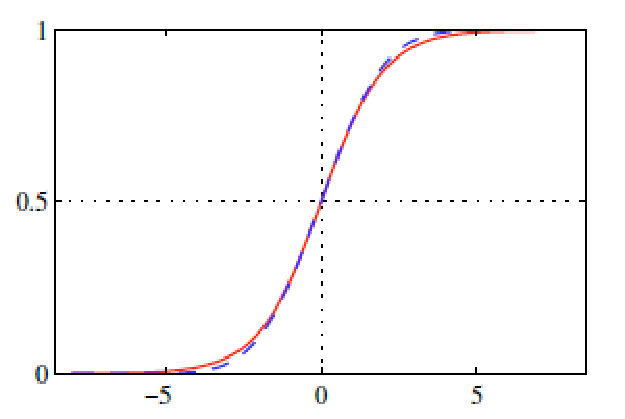
\includegraphics[scale=0.5]{figure/fig31.pdf}
\end{center}

Although the logistic sigmoid and the probit function arise from different motivations (one from the Bernoulli GLM with canonical link, the other from a Gaussian latent-threshold interpretation), they are qualitatively very similar: both are smooth sigmoids, both are symmetric around the origin, and both lead to linear decision boundaries in the feature space when a fixed threshold (e.g., $p=1/2$) is used for classification. Consequently, probit regression is usually employed in a way that is very close to logistic regression, and in many applications the two models yield nearly indistinguishable predictions once the coefficients are properly scaled.

%\medskip

\subsection*{Bayesian logistic regression}

%\subsubsection*{Bayesian logistic regression}

Up to now, learning in logistic regression has been presented as a point-estimation problem: we choose a single parameter vector $\w$ (for instance by maximum likelihood or MAP) and then plug it into $p({\cal C}_1\mid \x,\w)=\sigma(\w^{T}\overline\x)$. While this is often effective, it can lead to overfitting, especially when the dataset is small, features are high-dimensional, or classes are nearly separable. A Bayesian treatment addresses these issues by treating $\w$ as a random variable and by introducing a \emph{prior} distribution $p(\w)$ that encodes preference for plausible parameter values before seeing the data.

The key predictive quantity becomes the \alert{posterior predictive} probability, obtained by averaging the model prediction over the posterior uncertainty on $\w$:
\begin{align*}
p({\cal C}_{1}\mid\x,\X,\t)
&=\int p({\cal C}_{1}\mid\x,\w)\,p(\w\mid\X,\t)\,d\w\\
&=\int \sigma(\w^{T}\overline\x)\, p(\w\mid\X,\t)\,d\w,
\end{align*}
where, consistently with previous notation, $ \y=y(\x,\w)=\sigma(\w^{T}\overline\x)$.
This expression makes explicit a fundamental conceptual difference: predictions are no longer based on a single best $\w$, but on a distribution over plausible parameters, weighted by how compatible each $\w$ is with the observed data. In this way, uncertainty in parameter estimation is propagated into uncertainty in predictions, which is particularly valuable in ambiguous regions of the input space. Moreover, Bayesian averaging typically yields better-calibrated probabilities and can act as an automatic form of complexity control.

To compute this predictive distribution one needs a way to evaluate (or approximate) the posterior $p(\w\mid\X,\t)$.

\subsection*{Posterior distribution of coefficients}

By Bayes' rule, the posterior distribution of the parameters is
\begin{myequation}
p(\w|\X,\t)=\frac{p(\t|\X,\w)p(\w)}{p(\t|\X)}=
\frac{p(\t|\X,\w)p(\w)}{\int p(\t|\X,\w')p(\w')\,d\w'}.
\end{myequation}
Here $p(\t|\X,\w)$ is the likelihood of the training labels given inputs and parameters, and $p(\t|\X)$ is the \emph{evidence} (or marginal likelihood), which plays the role of a normalization constant ensuring that the posterior integrates to one.

Assuming conditional independence of training samples, the likelihood factorizes as
\begin{myequation}
p(\t|\X,\w)=\prod_{i=1}^{n}p(t_i\mid\x_i,\w),
\end{myequation}
with
\begin{myequation}
p(t_i|\x_i,\w)=
  \begin{cases}
   \sigma(\w^{T}\overline\x) & \text{if } t_i=1 \\
    1-\sigma(\w^{T}\overline\x) & \text{if } t_i=0.
  \end{cases}
\end{myequation}
This simply states that $t_i$ is modeled as a Bernoulli random variable with success probability $\sigma(\w^{T}\overline\x_i)$.

Using this Bernoulli form, the likelihood can be written compactly as
\begin{myequation}
p(\t|\X,\w)=\prod_{i=1}^{n}\sigma(\w^{T}\overline\x)^{t_i}\left(1-\sigma(\w^{T}\overline\x)\right)^{1-t_i}.
\end{myequation}
Substituting into Bayes’ rule yields
\begin{myequation}
p(\w|\X,\t)=\frac{p(\w)\prod_{i=1}^n\sigma(\w^{T}\overline\x)^{t_i}\left(1-\sigma(\w^{T}\overline\x)\right)^{1-t_i}}{Z},
\end{myequation}
where the normalization factor (the evidence) is
\begin{myequation}
Z=\int p(\w)\prod_{i=1}^n\sigma(\w^{T}\overline\x)^{t_i}\left(1-\sigma(\w^{T}\overline\x)\right)^{1-t_i} \, d\w.
\end{myequation}
The evidence has an important conceptual role: it measures how well the model class (including the prior) explains the data and it is central in Bayesian model comparison. In Bayesian logistic regression, however, it is also the main computational obstacle.

\subsection*{Predictive distribution intractability}

The difficulty is that $Z$ is typically hard (or impossible) to compute exactly in closed form. In practice, one is often only able to evaluate the unnormalized posterior,
\begin{myequation}
g(\w;\X,\t)=p(\w)\prod_{i=1}^n\sigma(\w^{T}\overline\x)^{t_i}\left(1-\sigma(\w^{T}\overline\x)\right)^{1-t_i},
\end{myequation}
which is proportional to $p(\w\mid\X,\t)$ through the unknown factor $Z$. This means that we can compare posterior values for different $\w$ (since $Z$ cancels out), but we cannot directly integrate or normalize without further approximations. Consequently, the posterior predictive integral
\begin{myequation}
p({\cal C}_{1}\mid\x,\X,\t)=\int \sigma(\w^{T}\overline\x)\,p(\w\mid\X,\t)\,d\w
\end{myequation}
is also generally intractable.

There are several standard strategies to cope with this intractability. One possibility is to reduce the posterior to a single representative point (MAP), another is to approximate it with a simpler distribution (variational or Laplace), and a third is to approximate integrals by sampling (Monte Carlo methods):
\begin{enumerate}
  \item find a single value of $\w$ which maximizes $p(\w|\X,\t)$: this corresponds to the value which maximizes $g(\w;\X,\t)$ (this is the usual MAP approach);
  \item approximate $p(\w|\X,\t)$ with some other probability density which can be treated analytically (\emph{variational} approach);
  \item sample from $p(\w|\X,\t)$, knowing only $g(\w;\X,\t)$ (\emph{Monte Carlo} approach).
\end{enumerate}
Even when these methods differ in philosophy and computational cost, they share a common goal: produce a tractable approximation of the posterior predictive distribution.

\subsection*{Bayesian logistic regression: MAP}

A first, conceptually simple approximation consists in summarizing the posterior $p(\w\mid\X,\t)$ by its mode, that is, by the maximum a posteriori (MAP) estimate. To make this explicit, we choose a prior distribution for $\w$. A standard choice, which simultaneously favors small weights and leads to analytical convenience, is a Gaussian prior with mean $\Zero$ and diagonal covariance $\sigma^2\I$:
\begin{myequation}
p(\w)={\cal N}(\w|\sigma^2)=\frac{1}{(2\pi)^{\frac{D}{2}}\sigma^D}e^{-\frac{\w^T\w}{2\sigma^2}}.
\end{myequation}
This prior can be interpreted as a soft preference for solutions with limited norm $\|\w\|$; it is also directly connected to $\ell_2$ regularization in the frequentist setting.

Since the training set likelihood with respect to $\w$ is, as usual,
\begin{myequation}
p(\X,\t|\w)=\prod_{i=1}^{n}y_i^{t_{i}}(1-y_i)^{1-t_{i}},
\end{myequation}
where $y_i=y(\x_i,\w)=\sigma(\w^T\oX(\x_i))$,
the logarithm of the posterior becomes
\begin{align*}
\log p(\w|\X,\t)
=&-\frac{1}{2\sigma^2}\w^T\w
+\sum_{i=1}^{n}\left(t_{i}\log y_i+(1-t_{i})\log (1-y_i)\right)+c.
\end{align*}
Thus, the MAP estimate balances data fit (the log-likelihood term) and complexity control (the quadratic prior term). The MAP value for $\w$ can be found, for example, by applying Newton--Raphson (the gradient and the Hessian matrix can be easily derived), exactly as in the non-Bayesian case but with an additional contribution due to the prior.

\subsection*{Bayesian logistic regression: Laplace approximation}

While MAP provides a single point estimate, a Bayesian approach is most meaningful when it retains at least some information about uncertainty. The \alert{Laplace approximation} addresses this by approximating a generic distribution $p(\z)$ with a Gaussian density $q(\z\mid\Vmu,\VSigma)$ centered at a mode of $p(\z)$, with covariance chosen to match the local curvature around that mode.

\begin{center}
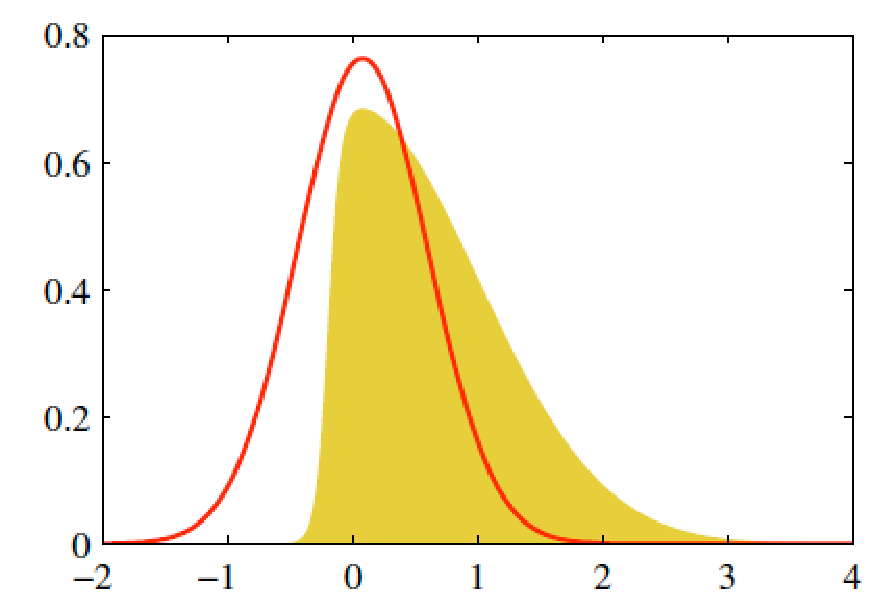
\includegraphics[scale=0.5]{figure/fig30.pdf}
\end{center}

Intuitively, the approximation relies on the idea that many posterior distributions are sharply peaked around their maxima when the dataset is informative. In such cases, a Gaussian can provide a good local approximation, and it yields tractable integrals for many quantities of interest.

\subsubsection*{Laplace approximation for $d=1$}

Consider first the one-dimensional case. Let
\begin{myequation}
p(z)=\frac{1}{Z}f(z),
\qquad
Z=\int f(z)\,dz,
\end{myequation}
where $Z$ is an unknown normalization constant. A mode (i.e., a maximum) $z_0$ of $p(z)$ is also a mode of $f(z)$, and it can be found by solving
\begin{myequation}
0=\frac{df(z)}{dz}.
\end{myequation}
A Gaussian distribution has a single mode, which coincides with its mean $\mu$. In Laplace approximation we therefore set the mean of the approximating Gaussian equal to the mode of $f$, i.e., $\mu=z_0$.

Moreover, $\log q(z)$ is a quadratic function:
\begin{myequation}
\log q(z)=-\frac{1}{2\sigma^{2}}(z-\mu)^{2}+c.
\end{myequation}
The central step is to approximate $\log f(z)$ itself by a quadratic function around $z_0$, so that $f(z)$ becomes approximately Gaussian in a neighborhood of the mode.

Consider the first two terms of the Taylor series expansion of $\log f(z)$ around $z_0$:
\begin{myequation}
\log f(z)\simeq \log f(z_{0})+\frac{d\log f(z)}{dz}\Bigg|_{z=z_{0}}\!\!\!\!\!\!\!\!\!\!(z-z_{0})
+\frac{1}{2}\frac{d^{2}\log f(z)}{dz^{2}}\Bigg|_{z=z_{0}}\!\!\!\!\!\!\!\!\!\!(z-z_{0})^{2}.
\end{myequation}
Since $z_0$ corresponds to a maximum of $f(z)$ and therefore also of $\log f(z)$, the first derivative term vanishes:
\begin{myequation}
\frac{d\log f(z)}{dz}\Bigg|_{z=z_0}\!\!\!\!\!\!\!\!\!\!=0.
\end{myequation}
Hence we obtain
\begin{myequation}
\log f(z)\simeq \log f(z_{0})-\frac{1}{2}A(z-z_{0})^{2},
\end{myequation}
where
\begin{myequation}
A=-\frac{d^{2}\log f(z)}{dz^{2}}\Bigg|_{z=z_{0}}.
\end{myequation}
By comparing the quadratic forms of $\log q(z)$ and $\log f(z)$, we identify
\begin{myequation}
\sigma^{2}=\frac{1}{A}.
\end{myequation}
Thus, the variance of the approximating Gaussian is given by the inverse curvature of $-\log f$ at the mode: sharper peaks correspond to smaller variance, encoding greater certainty.

Overall, we obtain
\begin{myequation}
q(z)=C e^{-\frac{A}{2}(x-z_{0})^{2}},
\end{myequation}
and, since $C$ is the normalization factor of a Gaussian,
\begin{myequation}
q(z)=\frac{\sqrt{A}}{\sqrt{2\pi}}e^{-\frac{A}{2}(x-z_{0})^{2}}.
\end{myequation}

\subsubsection*{Laplace approximation for $d>1$}

The multivariate case follows the same logic, but now the quadratic approximation involves matrices. Let $\z\in\mathbb{R}^{d}$ and let $\z_0$ be a mode of $f(\z)$, characterized by
\begin{myequation}
\frac{\partial f(\z)}{\partial \z}\Bigg|_{\z=\z_0}\!\!\!\!\!\!\!\!\!\!=0.
\end{myequation}
A second-order Taylor expansion of $\log f(\z)$ around $\z_0$ yields
\begin{myequation}
\log f(\z)\simeq \log f(\z_{0})-\frac{1}{2}(\z-\z_{0})^{T}\A(\z-\z_{0}),
\end{myequation}
where the matrix $\A$ is the Hessian of $-\log f(\z)$, evaluated at $\z_0$:
\begin{myequation}
\A=-\frac{\partial^2 \log f(\z)}{\partial\z^2}\Bigg|_{\z=\z_{0}}\!\!\!\!\!\!\!\!\!\!=\H(-\log f(\z))\Bigg|_{\z=\z_{0}}.
\end{myequation}
Then,
\begin{myequation}
f(\z)\simeq f(\z_0)e^{-\frac{1}{2}(\z-\z_{0})^{T}\A(\z-\z_{0})}
\quad \text{around } \z_0.
\end{myequation}
By setting the covariance matrix of the Gaussian approximation equal to $\A^{-1}$, we get
\begin{myequation}
q(\z)=Ce^{-\frac{1}{2}(\z-\z_{0})^{T}\A(\z-\z_{0})},
\end{myequation}
which, by normalizing, results into
\begin{myequation}
q(\z)=\frac{|\A|^{\frac{1}{2}}}{(2\pi)^{\frac{d}{2}}}e^{-\frac{1}{2}(\z-\z_{0})^{T}\A(\z-\z_{0})}.
\end{myequation}
As in the scalar case, directions in parameter space with strong curvature correspond to small posterior variance and therefore to well-determined combinations of parameters.

\subsection*{Applying Laplace approximation to Bayesian logistic regression}

If we apply Laplace approximation to $p(\w|\X,\t)$, we obtain a Gaussian distribution ${\cal N}(\w \mid \overline{\w}, \overline{\VSigma})$ such that
\begin{itemize}
\item ${\overline\w}=\w_{MAP}$ is computed as sketched before;
\item ${\overline\VSigma}$ is defined as
\begin{myequation}
{\overline \VSigma}=-\frac{\partial^2}{\partial\w^2}\log p(\w|\X,\t)
=\VSigma_{0}^{-1}+\sum_{i=1}^{n}y_i(1-y_i)\x_i\x_i^{T}.
\end{myequation}
\end{itemize}
The expression above makes explicit how prior information and data information combine: $\VSigma_0^{-1}$ (the prior precision) contributes a baseline curvature that prevents the posterior from becoming too flat, while the data term $\sum_i y_i(1-y_i)\x_i\x_i^T$ mirrors the Hessian structure of logistic regression and captures how informative each observation is about the parameters.

However, even after replacing the posterior by a Gaussian approximation, the predictive distribution remains difficult to compute analytically:
\begin{myequation}
p({\cal C}_{1}|\x, \X, \t)=\int \sigma(\w^T\Phi(\x))p(\w|\X, \t)d\w
\simeq \int y(\x,\w){\cal N}(\w|{\overline\w},{\overline\VSigma})d\w.
\end{myequation}
This integral is a convolution of a sigmoid with a Gaussian distribution and, in general, it does not admit a closed-form expression.

Two common routes can be followed. One possibility is to apply a further analytical approximation. Under suitable assumptions, one arrives at
\begin{myequation}
p({\cal C}_{1}|\x,\X,\t)\simeq\sigma\left(\frac{\w^T_{MAP}\overline\x}{\sqrt{1+\frac{\pi}{8}\overline\x^T\overline{\VSigma}\overline\x}}\right).
\end{myequation}
This expression can be interpreted as a \emph{shrinkage} of the effective margin $\w_{MAP}^{T}\overline\x$ by a factor that increases with predictive uncertainty $\overline\x^T\overline{\VSigma}\overline\x$. When the posterior over parameters is highly uncertain in directions relevant to $\overline\x$, the model becomes more conservative and produces probabilities closer to $1/2$.

A second alternative is to approximate the predictive expectation by sampling. One draws $N_s$ parameter vectors $\w_i$ from $p(\w|\X,\t)$ (or from an approximation of it), evaluates $\sigma(\w_i^{T}\overline\x)$ for each sample, and averages:
\begin{myequation}
p({\cal C}_{1}|\x,\X,\t)\simeq \frac{1}{N_s}\sum_{i=1}^{N_s}\sigma(\w_i^{T}\overline\x).
\end{myequation}

\subsection*{Bayesian logistic regression: MCMC sampling}

In the sampling-based approach, one would ideally sample directly from the true posterior $p(\w|\X,\t)$, rather than from its Gaussian approximation. The predictive distribution is still approximated as
\begin{myequation}
p({\cal C}_{1}|\x,\X,\t)\simeq \frac{1}{N_s}\sum_{i=1}^{N_s}\sigma(\w_i^{T}\overline\x),
\end{myequation}
but now the samples $\{\w_i\}_{i=1}^{N_s}$ are drawn from the exact posterior. Since $p(\w|\X,\t)$ is typically known only up to proportionality via $g(\w;\X,\t)$, this is precisely the setting in which \alert{Markov Chain Monte Carlo} (MCMC) methods are useful.

In MCMC, one constructs a Markov chain whose stationary distribution is the target posterior $p(\w|\X,\t)$. After an initial burn-in period, the states of the chain can be regarded as (dependent) samples from the posterior. Classical algorithms in this family include Metropolis--Hastings and Gibbs sampling. More advanced variants can exploit gradient information to improve efficiency in high-dimensional parameter spaces, but the essential principle remains the same: sampling enables Bayesian averaging without requiring closed-form normalization constants.

The practical advantage of MCMC is that it approximates the Bayesian predictive distribution without committing to a restrictive parametric approximation of the posterior. The corresponding cost is computational: obtaining sufficiently many effectively independent samples may require careful tuning and substantial runtime, especially when the posterior is highly correlated or multi-modal.





%\end{document}